\documentclass[twocolumn,twoside]{article}

\usepackage{graphicx}
\graphicspath{{./graphs/}{./drawn_images/}}
\usepackage{enumerate}


\title{\vspace{0.2cm}\huge\bf Report\vspace{1.2cm}}

\setlength{\textwidth}{15cm}
\setlength{\textheight}{22cm}
\setlength{\parskip}{0.5mm}
\setlength{\headheight}{0cm}
\setlength{\topmargin}{0cm}
\setlength{\headsep}{0cm}
\setlength{\oddsidemargin}{0cm}
\setlength{\evensidemargin}{0cm}
\renewcommand{\thesection}{\Roman{section}}


\author{
			{\normalsize \bf Sayan Mitra, Surajeet Bharati, Sushmita Sen}\\
			{\small \textit{Department of Computer Science and Technology}}\\
			{\small \textit{IIEST, Shibpur, Howrah - 03}}\\
			{\small \textit{Email :- \{sayan.besu,surajeet01,sushmita.sen.edu\}@gmail.com }}\\
			\and
			{\normalsize \bf Anupam Chandra, Niramlya Chatterjee, Abhishek Mukhopadhyay}\\
			{\small \textit{Department of Computer Science and Technology}}\\
			{\small \textit{IIEST, Shibpur, Howrah - 03}}\\
			{\small \textit{Email :- \{anupamchanda2011,nirmalya.besucst,toct92\}@gmail.com }}
}
\date{}

\begin{document}
		\maketitle

		{\bf \textit{Abstract} - Automatic Categorization of a movie is the task of categorizing the movie into a specific group like Action, Horror, Comedy or Drama without watching the whole movie, even without opening the movie into some media player. Besides, one can be interested only to some specific scenes of the movie. So, in place of the movie, he should be presented with a small number of most important frames that will be representative of the whole movie. Using these small number of key frames, one can also guess about the category or jump to some specific location that he wants to watch. Our objective is to process a movie and automatically extract those desired frames.}
		
		
		
		\vspace{0.3cm}
		{\bf \textit{Keywords} - Video Processing, Movie Category, Key frames}
		
		
		\vspace{0.7cm}
		\begin{center}
		    {\large 1. INTRODUCTION}
		\end{center} 
		\vspace{0.3cm}
			
    We were going to extract most important key frames of a input movie. For this purpose, first of all we have to extract the key frames of each and every shot. A shot is a continuous sequence or footage between two edits or cuts. So, we have to determine the boundaries (frame number) of all the shots of the movie. For this, We have to divide all the frames of the movie, determine differences between consecutive frames with respect to total pixel information of the frames and with respect to those difference values and considering a predefined threshold value, we can obtain the shot boundaries in the movie. So, we have to first determine a universal threshold value for which we will get maximum success rate for all types of movies. We followed two different methods to determine the threshold value and later to determine shot boundaries. After extracting all key-frames, we have to remove most similar frames (that can happen when a conversation is going on throughout a scene) reducing the number of frames to a much smaller number. To perform this reduction, we used some clustering or spanning tree algorithm.\\
		
		
		\vspace{-0.6cm}
		\begin{center}
		    {\large 2. PROPOSED APPROACH}
		\end{center} 
		\vspace{-0.5cm}
		
We followed two different approaches to determine the threshold. One approach is calculating average absolute difference of frequency tables of pixel values of each two consecutive frames. In the other case, we calculated average of square of motion vectors that was determined by different motion Estimation algorithms. \\   
		
		\vspace{3cm}
		{\normalsize 2.1. AVERAGE ABSOLUTE DIFFERENCE BETWEEN FREQUENCY VECTORS OF CONSECUTIVE FRAMES}\\ \\
		
The steps followed in this approach are elaborated here one by one.\\
		
		\textit{A. Manually identifying boundary of each shot :}\\
		
		We have to first determine a threshold value to make the whole thing working. So, we first started calculating threshold value for four movies namely Taken (Action), Mr. Bean (Comedy), The Conjuring (Horror) and My Sassy Girl (Drama). Those movies are first divided into its constituent frames using Matlab or any other video to jpeg converter. We then manually identified every frame number where a new shot started and enlisted them.\\ 
		
		\vspace{0.4cm}
		\textit{B. Calculating frequency vectors for every frames : }\\ 
		
		Every frame is converted to R-G-B frames. For each component (R,G,B) there will be a matrix of size $FrameHeight\times FrameWidth$ with values of each element between 0 to 255. For each of these matrix, we calculated frequency vectors of size $1\times 256$. Then the main frame is converted to $YC_bC_r$ frame. Taking the Y component, absolute differences between each two consecutive rows and differences between each two consecutive columns produce two more matrixes of size $FrameHeight-1\times FrameWidth$ and $FrameHeight\times FrameWidth-1$ respectively. Two more frequency vectors are calculated from this two matrixes. 
			
\vspace{0.3cm}

So we get total five frequency vectors. Merging these five vectors, we got the frequency vector of size $1\times 1280$. We then divided each element of the vector with number of pixels in a frame of the movie and as it produced too much small values,for clarity we multiplied all the elements with 100000. This vector is the final frequency vector for each of the frames. We took this vector as the representation of the frame.\\


		\textit{C. Calculating Differences between the frames:}\\
		
		We then go on calculating differences for consecutive frame taking the average of the difference between frequency vectors and storing them in two files - one for all frames in same shot and the other contains shot changing frames. Two sets of frames of same and different shots with their averaged difference are shown in figure.1 and figure.2.
		
		\vspace{0.1cm}
		\begin{center}
				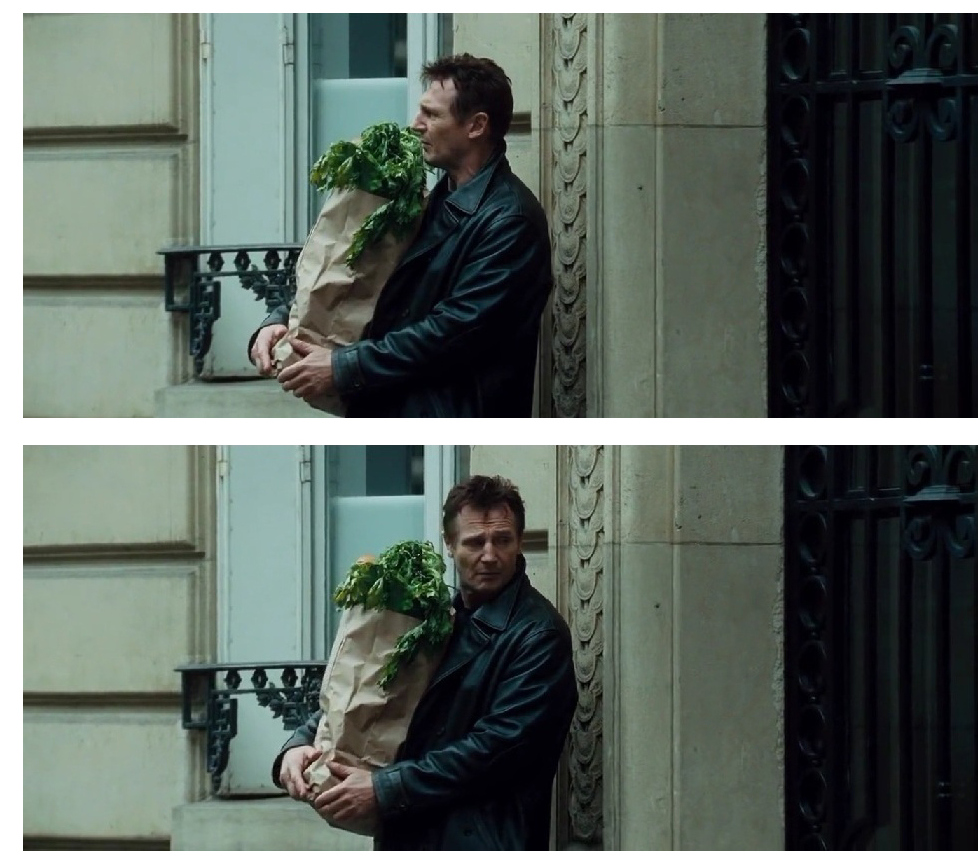
\includegraphics[scale=0.2]{sameshot}
		\end{center}
		\vspace{-0.6cm}
		\begin{center}
				{\tiny Figure 1: Frames of a Same Shot with Difference = 21}
		\end{center}
		\vspace{0.1cm}
		\begin{center}
				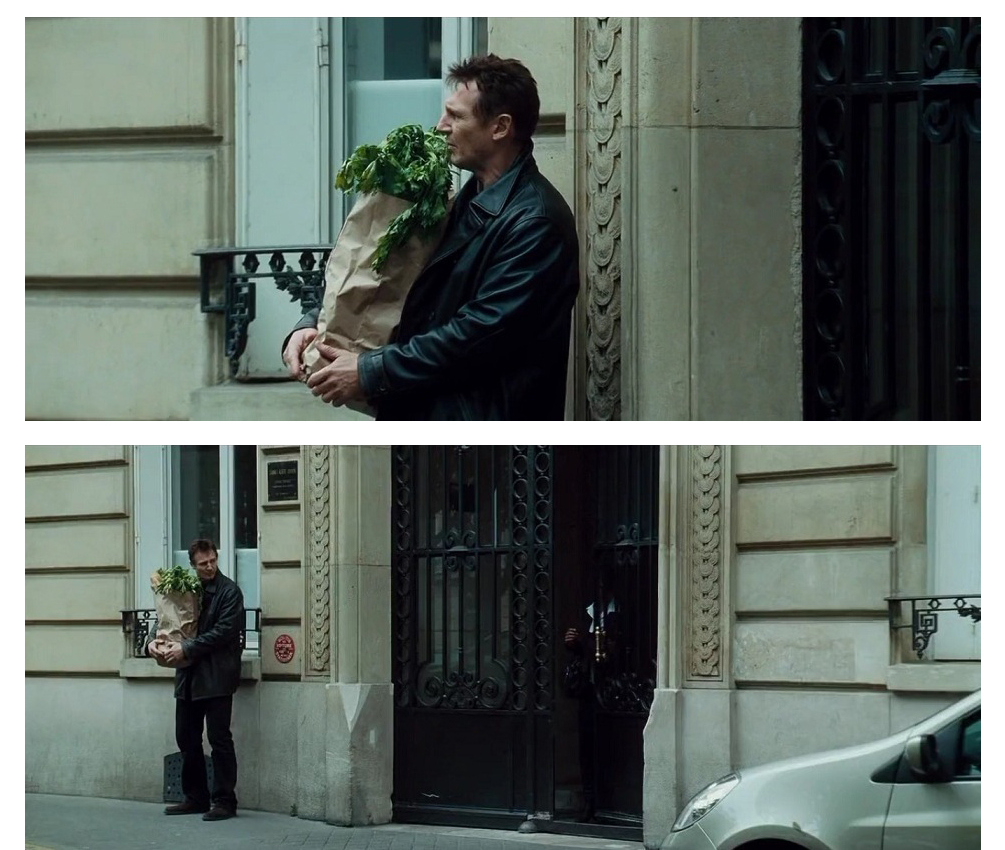
\includegraphics[scale=0.2]{diffshot}
		\end{center}
		\vspace{-0.6cm}
		\begin{center}
				{\tiny Figure 2: Frames of different Shots with Difference = 130}
		\end{center}
		\vspace{0.2cm}

 We saw that the difference between the frames of same shot was smaller compared to the difference of shot changing frames. So, this variation of differences lead us to the idea of breaking frames into groups of same shot and different shot by finding a threshold value for difference and thus,automate our manual sorting technique of making groups of frames.\\

		\vspace{0.4cm}
		\textit{D. Calculating Threshold Value of Difference :}\\ 
		
	We already had the boundaries for every shot of each of the movies. With help of these, we got two different set of differences for each of the movies. Then, we calculated Threshold from each of the three movies and applied that value to the fourth movie.\\
		
		
		\begin{center}
				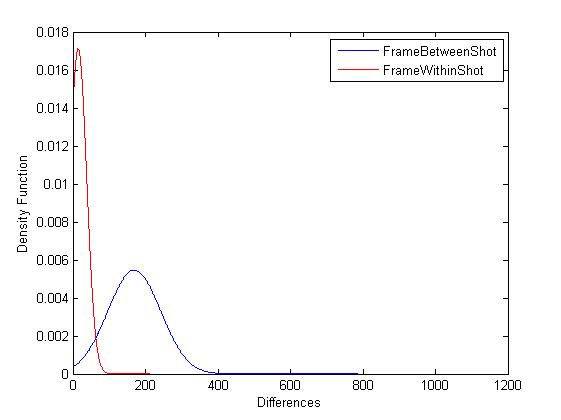
\includegraphics[scale=0.4]{taken_97}
		\end{center}
		\vspace{-0.6cm}
		\begin{center}
				{\tiny Figure 3: For movies Mr. Bean,The Conjuring,My Sassy Girl}
		\end{center}
		\begin{center}
				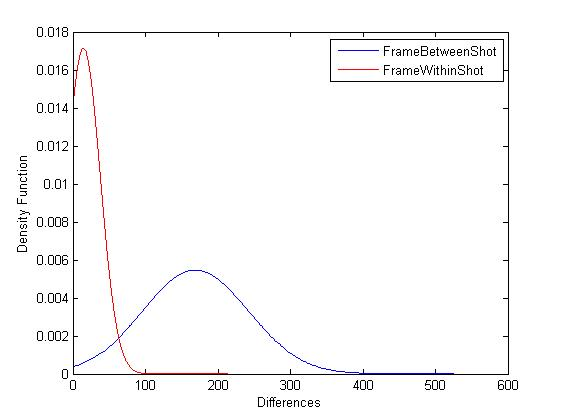
\includegraphics[scale=0.4]{sassy_girl_96}
		\end{center}
		\vspace{-0.6cm}
		\begin{center}
				{\tiny Figure 4: For movies Mr. Bean,The Conjuring,Taken}
		\end{center}
		\vspace{0.3cm}
		
		
		We merged the three sets of differences for frames of same shots and three sets of differences for frames between shots. Using Chi
Squared Test, We found that the Probability Density Function for same shot frame differences and shot changing frame differences follow normal distribution having different mean and standard derivation that intersect and have some common area under the curve.

		\begin{center}
				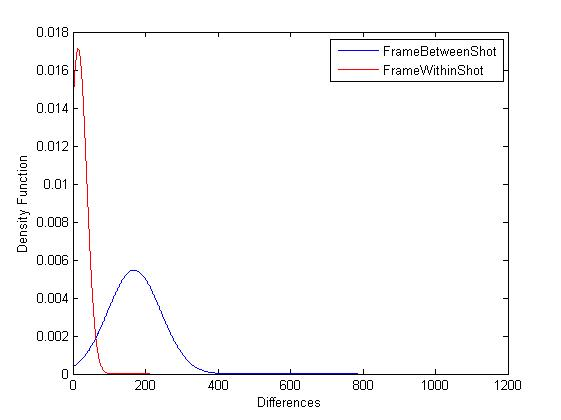
\includegraphics[scale=0.4]{bean_97}
		\end{center}
		\vspace{-0.6cm}
		\begin{center}
				{\tiny Figure 5: For movies Taken,The Conjuring,My Sassy Girl}
		\end{center}
		\begin{center}
				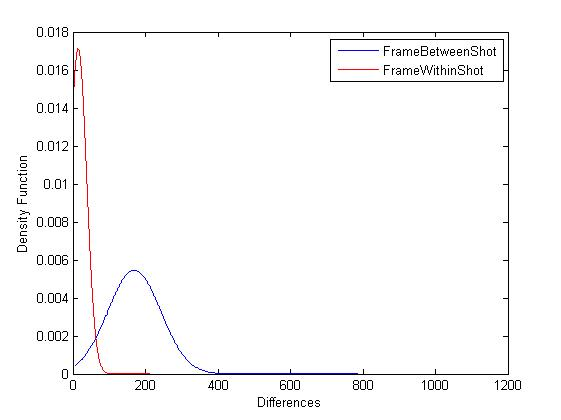
\includegraphics[scale=0.4]{conjuring_97}
		\end{center}
		\vspace{-0.6cm}
		\begin{center}
				{\tiny Figure 6: For movies Mr. Bean,My Sassy Girl,Taken}
		\end{center}
		
	 We seek to find the threshold value of the average difference of probability (the one we stored and built the PDF graph) which will act as a measure to divide the frame automatically and serve as a way to automate our manual sorting technique of the frames.\\ 

	Since,the Normal Probability Density Function's of the two sets have intersecting  area, we can't usually tell the threshold value. We iteratively picked a value in the range of intersecting probabilities and calculate the error by finding the weighted area under the curve for the two Probability Density Function's. The point which gives the least error is chosen as the threshold value. \\

$error =  \int_{-\infty}^x P_1\left(x\right) . P_1 + \int_x^{\infty} P_2\left(x\right) . P_2$ \\

\vspace{0.1cm}
where $x$ is a picked value, $P_2$ and $P_1$ are the probability of the respective frames from the set for frames within same shots and frames between two different shot respectively are selected, $P_1\left(x\right)$ and $P_2\left(x\right)$ are probability density functions for the set of frames within shot and set of frames between shot respectively.\\

\vspace{0.1cm}
For the different combination of three movies we got almost same threshold values that were 97(for Figure.3), 96(for Figure.4), 97(for Figure.5), 97(for Figure.6) and get over $95\%$ success in case of automatically calculating boundaries for fourth movie. Then we calculated threshold by merging all sets for four movies and get threshold value 97 and get over $95\%$ success for all the four movies applying this value as threshold. So, we decided to take \emph {97} as the universal threshold value to be used in future for every other movie. \\ \\

		\vspace{0.2cm}
		\textit{E. Extracting key frames for all shots :}\\ \\
		
		After breaking the movie into groups of same shot frames using the above method, we found the key frame of each group by the following algorithm, building on the idea that the average vector is a good representation of the entire group and the frame in the group closest to it will be the key frame for that group. 
\vspace{0.1cm}

\begin{enumerate}[i]
		\item {For each frame in the same shot, we added this components vectors and took the average vector and stored it.}
		\item {Now, we iteratively took each frame of the group and calculated the difference of it's vector with the average vector found above.}
		\item {The frame which give the minimum difference is chosen as the key frame.}
\end{enumerate}

Since, the number of key-frames can be large, talking all of them to represent the movie may not be suitable. So, we have to remove similar frames and extract most distinct key frames.\\


		\vspace{0.4cm}
		\textit{F. Extracting most distinct key frames :}\\ \\ 
		
To reduce the number of key frames to $K$ from $N$ where K is much smaller than N, firstly we calculated differences between each two frames by the process said before. We got total n(n-1)/2 number of differences. We designed two different algorithm to get K frames --\\ \\
		\vspace{0.1cm}
a) By using spanning tree - 
		A spanning tree have to be first implemented whose N number of nodes represent N frames. All nodes have to be connected to each other. So, initially there is a single connected tree. Now, we have to identify the two frames between which difference is maximum. The nodes representing these two frames are then disconnected. After that, we have to identify those two frames between which difference is second maximum and there nodes have to be disconnected. Same process have to be followed until there remain K number of connected trees. Then, following the process of extracting a key frame from all the frames of a shot, one frame have to extracted from each of the connected set of the frames.\\

b) By using clustering Algorithm - 
		In this case, Union-Find data structure is used. Initially, there will be N number of sets each containing one key frame. Now, as before considering the n(n-1)/2 difference values already calculated, we have to identify the frames within which the difference is minimum. Now, sets that contain those frames, have to be merged (Union Operation).  Same process have to be followed for second minimum difference value and so on. This process have to be continued until K number of sets last. Then, from each set, one frame have to be exacted following the process said before.
		
		
\vspace{3cm}
		
{\normalsize 2.2. MOTION ESTIMATION ALGORITHMS TO CALCULATE DIFFERENCES BETWEEN CONSECUTIVE FRAMES}\\ \\

Another method of sorting the frames into groups of same shots and different shots is using block matching techniques. A block matching algorithm gives the motion vector of all blocks (i.e. the displacement of the center of a square of pixels of predetermined dimensions when a frame changes to another frame). The displacement of a block in present frame in any general block matching algorithm is found by comparing each pixel value of each block in previous frame. The block in previous frame with minimum different in pixel values is chosen as the representation of the present block, the displacement being the difference of ($x,y$) coordinate of the centres of these two blocks.\\

Now, the present frame is built from the previous frame by replacing the blocks in present frame with closest matching blocks in previous frame. The difference between the newly built present frame and the original present frame is found by the previous technique of using the representative vector of frames and taking the averaged probability difference.\\

The successive differences in frames using this block matching technique is stored. The idea of grouping frames into same and different shots is that consecutive frames in same shot differ only slightly in appearance, i.e most of the blocks in present frame matches exactly with previous frame and hence difference between the newly constructed frame and present frame is small compared to frames of different shots where most of the blocks don't match and the error/difference using the patching is greater. We plan to find the threshold difference value and check its success against the previous method with the notion that this being a superior technique as it operates on pixel value level, will give some accurate results.\\

Some of the block matching algorithms that we used are: 
\begin{enumerate}[i]

\item {\textit {Three Step Search} (TSS) : It starts with the search location at the center and sets the ‘step size’ S = 4, for a usual search parameter value of 7. It then searches at eight locations +/- S pixels around location (0,0). From these nine locations searched so far it picks the one giving least cost and makes it the new search origin. It then sets the new step size S = S/2, and repeats similar search for two more iterations until S = 1. At that point it finds the location with the least cost function and the macro block at that location is the best match. The calculated motion vector is then saved for transmission.}\\

\item {\textit {New Three Step Search} (NTSS) : In NTSS first of all the cost points are checked in addition to the search origin(point) for minimum weight. Totally there will be 17 points considering origin. The additional search locations, that is 8 are a distance of S = 4 away and the other 8 points are at S = 1 away from the origin then the search is stopped suddenly. Then the motion vector is set to as (0,0). The search pattern in NTSS for each step is fixed. NTSS is very much compatible with the TSS in terms of computational complexity. The NTSS algorithm differs from TSS in 2 aspects. Firstly, they are used a center-biased checking point pattern in its first step, in order to make the search adaptive with the distribution of motion vector. Secondly, added a halfway-stop technique for stationary blocks or quasi-stationary blocks.}\\

\item {\textit {Four Step Search} (4SS) : Similar to NTSS, 4SS also employs center biased searching and has a halfway stop provision. 4SS sets a fixed pattern size of S = 2 for the first step, no matter what the search parameter p value is. Thus it looks at 9 locations in a $5\times 5$ window. If the least weight is found at the center of search window the search jumps to fourth step. If the least weight is at one of the eight locations except the center, then we make it the search origin and move to the second step. The search window is still maintained as $5\times 5$ pixels wide. Depending on  where the least weight location was, we might end up checking weights at 3 locations or 5 locations. The patterns are shown in Fig 7. Once again if the least weight location is at the center of the $5\times 5$ search window we jump to fourth step or else we move on to third step. The third is exactly the same as the second step. IN the fourth step the window size is dropped to $3\times 3$, i.e. S = 1. The location with the least weight is the best matching macro block and the motion vector is set to point o that location. A sample procedure is shown in Fig 8. This search algorithm has the best case of 17 checking points and worst case of 27 checking points.}\\

\item { \textit {Diamond Search} (DS) : DS algorithm is exactly the same as 4SS, but the search point pattern is changed from a square to a diamond, and there is no limit on the number of steps that the algorithm can take. DS uses two different types of fixed patterns, one is Large Diamond Search Pattern (LDSP) and the other is Small Diamond Search Pattern (SDSP). These two patterns and the DS procedure are illustrated in Fig. 9. Just like in FSS, the first step uses LDSP and if the least weight is at the center location we jump to fourth step. The consequent steps, except the last step, are also similar and use LDSP, but the number of points where cost function is checked are either 3 or 5 and are illustrated in second and third steps of procedure shown in Fig.9. The last step uses SDSP around the new search origin and the location with the least weight is the best match. As the search pattern is neither too small nor too big and the fact that there is no limit to the number of steps, this algorithm can find global minimum very accurately. The end result should see a PSNR close to that of ES while computational expense should be significantly less.}

\end{enumerate} 

\vspace{0.5cm}

These algorithms differ mostly in computation complexity, giving us motion vector ($x,y$) displacement vector for each block of frame. We then apply our the technique mentioned above.\\

We used two different approaches to calculate differences between two successive frame using above said motion estimation algorithms.\\\\
 
2.2.1. To calculate difference between frame no n and frame no (n+1) , firstly both the frames are divided into equal number of equal sized blocks. Then in frame no n, around i-th block, a search area is created. In this search area ,we searched for i-th block of(n+1)-th frame. The original i-th block in (n+1)-th frame is replaced by the matching block. In this way, all the blocks of (n+1)-th is frame is replaced and a new frame is created. We have to then calculate difference between the original (n+1)-th frame and the modified (n+1)-th frame (created by replaced matching blocks) by calculating the frequency table of both the frames and then calculating the frequency table of both the frames and then calculating their average absolute difference . This process has been discussed in Section 2.1.\\

\begin{center}
		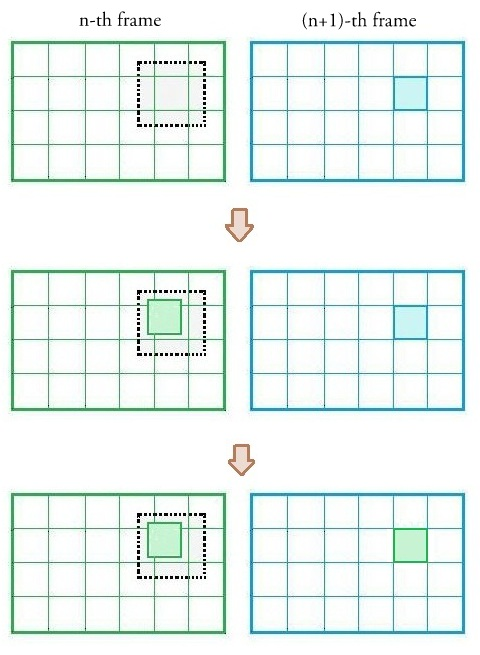
\includegraphics[scale=0.3]{final}
\end{center}
\vspace{-0.8cm}
\begin{center}
		{\tiny Figure 7: Block replacing process}
\end{center}
\vspace{0.2cm}

Following this process we get the differences between each two consecutive frames. After thoroughly observing the set of difference we observed that the characteristics of that set matches with the set of differences calculated by the 1st approach. Difference between two frames in same shot is much smaller than difference between two frame of different shot as before. This observation give us the idea that this approach can also be used to achieve our target.\\                
		 	
Using Chi-Squared Test, We observed that this set of difference is also in normal distribution and we get same type of probability distribution graph as we saw in case of our previous approach.\\
So, We reached to the decision that this approach can also be used to calculate a universal threshold and using that we can automate the process of identifying the shot boundaries.\\ \\
2.2.2. In this case also , as before each of the n-th and (n+1)-th frame is divided into some numbers of equal sized blocks and a search area is created around the i-th block of n frame . Using motion estimation algorithms, We get motion vectors for (n+1)-th frame with respect to n-th frame for each block .For m number of blocks we got m number of motion vector co-ordinate pair (u,v). We calculated average of $u^2$ and $v^2$. This average squared value pair is considered as the difference between the two consecutive frames. This set of differences again follow the characteristics  of the set of differences calculated using two procedures discussed before . So, in this case, we also can fix a threshold  value to automatically identify the frame numbers where a new shot starts.

\end{document}